\begin{solution}
\begin{enumerate}
\item {[4 points]} The best approximation to $f(x) = \cos(\pi x)$ from ${\rm span}\{\phi_1\}$ with respect to the norm $\norm{\cdot}$ is
       \[ f_1(x) = {(f,\phi_1) \over (\phi_1, \phi_1)} \phi_1(x).\]
In Homework 16 we computed that
\[
          \ip{\phi_1,\phi_1} =2.
\]
Moreover, we can compute that
\[
          \ip{f,\phi_1} = \int_{-1}^1 \cos(\pi x)\,dx = \left[\frac{1}{\pi}\sin(\pi x)\right]_{-1}^1=\frac{1}{\pi}\sin(\pi)-\frac{1}{\pi}\sin(-\pi)=0-0=0
\]
and hence
       \[ f_1(x) = 0.\]
\\
\item {[7 points]} Since $\phi_1$ and $\phi_2$ are
      orthogonal with respect to the inner product $\ip{\cdot,\cdot}$, i.e., $\ip{\phi_1, \phi_2} = 0$, the best approximation to $f(x) = \cos(\pi x)$ from ${\rm span}\{\phi_1,\phi_2\}$ with respect to the norm $\norm{\cdot}$ is
       \[ f_2(x) = {(f,\phi_1) \over (\phi_1, \phi_1)} \phi_1(x) + {(f,\phi_2) \over (\phi_2, \phi_2)} \phi_2(x) = f_1(x) + {(f,\phi_2) \over (\phi_2, \phi_2)} \phi_2(x).\]
In Homework 16 we computed that
      \[
         \ip{\phi_2,\phi_2} = {2\over 3}.
\]
Moreover, we can compute that
\begin{eqnarray*}
\ip{f,\phi_2} &=&\int_{-1}^1 x\cos(\pi x)\,dx 
\\
&=&\left[\frac{1}{\pi}x\sin(\pi x)\right]_{-1}^1-\int_{-1}^1 \frac{1}{\pi}\sin(\pi x)\,dx 
\\
&=& \frac{1}{\pi}\sin(\pi)-\left(-\frac{1}{\pi}\sin(-\pi)\right)-\left[-\frac{1}{\pi^2}\cos(\pi x)\right]_{-1}^1 
\\
&=& \frac{1}{\pi^2}\cos(\pi)-\frac{1}{\pi^2}\cos(-\pi)
\\
&=&-\frac{1}{\pi^2}-\left(-\frac{1}{\pi^2}\right)
\\
&=&0
\end{eqnarray*}
and hence
       \[ f_2(x) = f_1(x)
                  + {(f,\phi_2) \over (\phi_2, \phi_2)} \phi_2(x) = 0.\]
\\
\item {[7 points]}
Since,
 \[ (\phi_1,\phi_2) = (\phi_1,\phi_3) = (\phi_2,\phi_3) = 0,\]
the best approximation to $f(x) = \cos(\pi x)$ from ${\rm span}\{\phi_1,\phi_2,\phi_3\}$ with respect to the norm $\norm{\cdot}$ is
       \[ f_3(x) = {(f,\phi_1) \over (\phi_1, \phi_1)} \phi_1(x) + {(f,\phi_2) \over (\phi_2, \phi_2)} \phi_2(x) + {(f,\phi_3) \over (\phi_3, \phi_3)} \phi_3(x) = f_2(x) + {(f,\phi_3) \over (\phi_3, \phi_3)} \phi_3(x).\]
In Homework 16 we computed that
\[
  \ip{\phi_3,\phi_3} = {8\over 5}.
\]
\\
Moreover, we can compute that
\begin{eqnarray*}
  \ip{f,\phi_3} &=& \int_{-1}^1 (3x^2-1)\cos(\pi x)\,dx
\\
 &=& 3\int_{-1}^1 x^2\cos(\pi x)\,dx-\ip{f,\phi_1}
\\
 &=& 3\int_{-1}^1 x^2\cos(\pi x)\,dx
\\
 &=& 3\left(\left[\frac{1}{\pi}x^2\sin(\pi x)\right]_{-1}^1-2\int_{-1}^1 \frac{1}{\pi}x\sin(\pi x)\,dx\right)
\\
 &=& 3\left(\frac{1}{\pi}\sin(\pi)-\frac{1}{\pi}\sin(-\pi)-\left[-\frac{2}{\pi^2}x\cos(\pi x)\right]_{-1}^1-\frac{2}{\pi^2}\int_{-1}^1 \cos(\pi x)\,dx\right)
\\
 &=& 3\left(-\left(-\frac{2}{\pi^2}\cos(\pi )-\frac{2}{\pi^2}\cos(-\pi)\right)-\frac{2}{\pi^2}\ip{f,\phi_1}\right)
\\
 &=& 3\left(-\frac{2}{\pi^2}-\frac{2}{\pi^2}\right)
\\
 &=& -\frac{12}{\pi^2}
\end{eqnarray*}
thus giving
       \[ f_3(x) = f_2(x) + {(f,\phi_3) \over (\phi_3, \phi_3)} \phi_3(x) = -\frac{15}{2\pi^2} (3x^2-1) .\]
\\
\item {[7 points]} The following plot compares the best approximations to $f(x)$. Note that $f_2$ obscures $f_1$.

\begin{center} 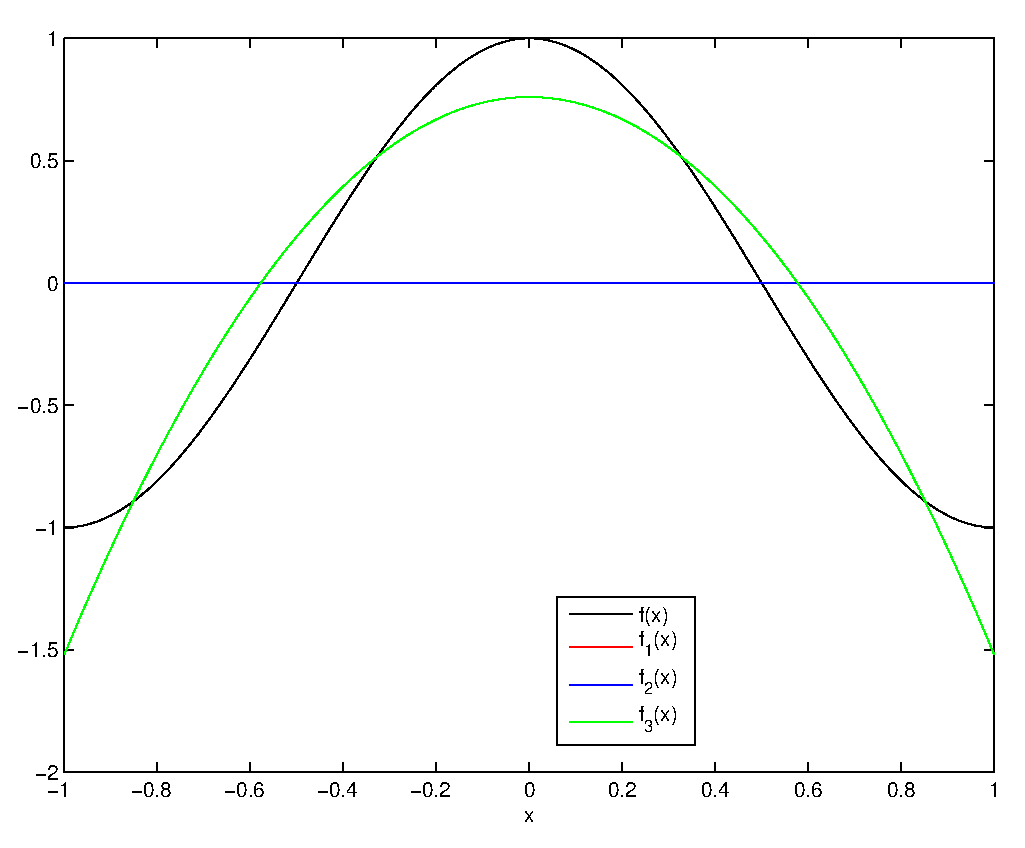
\includegraphics[scale=0.5]{hw17d} \end{center}

The code use to produce it is below.

\lstinputlisting{HW17d.m}
\end{enumerate}
\end{solution}

